\documentclass[../main.tex]{subfiles}
\begin{document}
\begin{center}
\begin{tabularx}{\textwidth}{|1|X|}
\hline
    Kratak opis &  Korisnik postaje član teretane tako što uz pomoć recepcionara popunjava formular sa ličnim podacima. Podaci se validiraju i korisnik dobija povratnu informaciju o uspehu registracije.\\ 
\hline    
    Učesnici & \begin{enumerate}
        \item Neregistrovani korisnik – Želi da postane član teretane kako bi mogao da koristi njegove usluge.
        \item Recepcionar – Želi da efikasno izvši registraciju novog korisnika na sistem.
     \end{enumerate}\\
\hline
   Preduslovi & \begin{enumerate}
       \item Sistem je u funkciji.
       \item Korisnik nije član teretane.
   \end{enumerate}\\
\hline  
    Postuslovi & \begin{enumerate}
        \item Korisniku je kreiran nalog.
        \item Baza podataka je ažurirana.
    \end{enumerate}\\
\hline
    Osnovni tok & \begin{enumerate}
        \item Korisnik dolazi na recepciju teretane i izjašnjava se da želi da postane član.
        \item Recepcionar u sistemu bira opciju za registraciju novog člana.
        \item Recepcionar pita korisnike za osnovne podatke i unosi ih u formular.
        \item Recepcionar nakon što su popunjena sva polja klikće na dugme „Registruj korisnika“.
        \item Sistem vrši proveru podataka.
        \item Sistem šalje e-mail sa podacima.
        \item Sistem obaveštava da je nalog aktiviran.
        \item Recepcionar obaveštava korisnika da je nalog uspesno kreiran.
        \item Recepcionar predaje korisniku člansku kartu korisniku.
    \end{enumerate}\\
\hline
    Alternativni tokovi & \begin{itemize}
        \item[A5] Neuspesna provera podataka: Recepcionar obaveštava korisnika koje polje nije ispravno. Nastavlja se na koraku 3.
    \end{itemize}\\
\hline
    Podtokovi & /\\
\hline
    Specijalni zahtevi & Korisnik mora da ima e-mail adresu.\\
\hline
    Dodatne informacije & Formular za registraciju od podataka zahteva: korisničko ime, ime, prezime, e-mail, broj telefona, lozinku, polje za proveru lozinke.\\
\hline
\end{tabularx}
\end{center}    

\begin{figure}[!ht]
\begin{center}
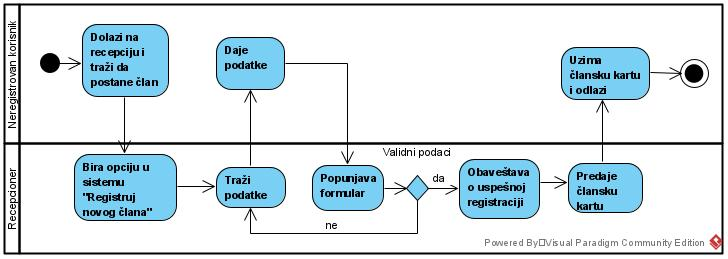
\includegraphics[scale=0.55]{sections/images/Dijagram_aktivnsti_registracije_uzivo.jpg}
\end{center}
\caption{Dijagram aktivnosti registracije uživo}
\label{fig:kontekst}
\end{figure}
\end{document}